\documentclass[10pt]{article}
\usepackage[a4paper, left=2cm, right=2cm, top=2.5cm, bottom=2.5cm]{geometry}
\usepackage{theme}
\usepackage{shortcuts}

\usepackage{graphicx}
\usepackage{amsmath,amssymb}
\usepackage{booktabs}
\usepackage{float}

\usepackage{algorithm}
\usepackage{algorithmicx}
\usepackage{algpseudocode}

\usepackage{titlesec}
\titlespacing*{\paragraph}
  {0pt}    % left indent
  {3pt}    % space BEFORE
  {3pt}

\usepackage[style=numeric]{biblatex}
\addbibresource{bibliography.bib}
\renewcommand*{\bibfont}{\normalfont\small}

% Document parameters
% Document title
\title{\vspace{-2cm}
      \LARGE{Biostatistics Paper Reading Assignment - MVA 2025/2026}
      \\ \large{A radiomics approach to assess tumour-infiltrating CD8 cells and response to anti-PD-1 or anti-PD-L1 immunotherapy: an imaging biomarker, retrospective multicohort study}
      }

\author{
Adonis JAMAL \email{adonis.jamal@student-cs.fr}
}

\date{\vspace{-5ex}}

% ==============================================================================
% ================================== DOCUMENT ==================================  
% ==============================================================================
\begin{document}
\maketitle


% ==============================================================================
% SECTION : INTRODUCTION AND CONTRIBUTIONS
% ==============================================================================
\section{Introduction and Contributions}
Immunotherapy, particularly the use of anti-programmed cell death protein 1 (PD-1) and anti-programmed cell death ligand 1 (PD-L1) checkpoint inhibitors, has revolutionized the treatment of advanced solid tumours. However, clinical success remains highly variable, with only $20\%$ to $50\%$ of patients exhibiting an objective response to these treatments \cite{chen2017elements}. Research has established that a patient's response is strongly correlated with their tumour's pre-existing immune phenotype; specifically, "immune-inflamed" tumours characterized by dense CD8+ cytotoxic T-cell infiltration tend to respond favorably, in stark contrast to "immune-desert" or "immune-excluded" phenotypes. Currently, assessing CD8 infiltration relies on invasive tumour biopsies evaluated via immunohistochemistry or RNA sequencing. These traditional standard-of-care methods inherently suffer from sampling bias, fail to capture spatial heterogeneity across the entire tumour microenvironment, and cannot be easily repeated for continuous, longitudinal monitoring. Furthermore, standard biomarkers such as PD-L1 expression have demonstrated inconsistent predictive reliability in recent randomized trials \cite{gandhi2018pembro}.

To overcome these limitations, Sun et al. \cite{main} proposed a non-invasive radiomics approach. Radiomics operates on the hypothesis that the high-dimensional quantitative features, such as texture, shape, and intensity, extracted from routine medical images reflect deeper cellular and molecular tissue properties. The primary objective of their study was to develop and independently validate a CT-based radiomic signature of tumour-infiltrating CD8 cells, and to subsequently evaluate its ability to predict immune phenotypes and clinical outcomes in patients receiving immunotherapy. The paper's main contribution to the field is the development of the first radiomics-based biomarker for CD8 infiltration validated across multiple independent cohorts, successfully bridging macroscopic imaging features with genomic expression, pathology, and survival outcomes.

In this report, our primary contribution is a critical appraisal of Sun et al.'s \cite{main} foundational study. We systematically review their methodology and experimental setup, evaluate the strengths and limitations of their data curation, and critically analyze the robustness of their results to highlight both the clinical promise and the methodological caveats of this imaging biomarker.


% ==============================================================================
% SECTION : METHODOLOGY
% ==============================================================================
\section{Methodology}
The core methodology of the paper centers on constructing a predictive bridge between macroscopic imaging features and microscopic genomic expression. The pipeline is divided into image segmentation, feature extraction, response variable definition, and model construction.

\subsection{Image Segmentation and Volumes of Interest (VOIs)}
To standardize the input data, the authors strictly selected contrast-enhanced CT scans with a slice thickness of $5$ mm or less, reconstructed using soft or standard convolution algorithms. Tumours were semi-automatically delineated by radiation oncologists using ISOgray software.

The authors did not restrict their analysis to the tumour alone. To capture quantitative data from the surrounding tumour microenvironment, where immune cells typically infiltrate, they generated a second VOI: a peripheral ring. This was created by automatically dilating and shrinking the tumour boundary by $2$ mm in both directions, resulting in a $4$ mm thick ring. Large vessels, adjacent organs, and air cavities were excluded if not infiltrated by tumour cells.

\subsection{Radiomic Feature Extraction}
Using LIFEx software, the images underwent preprocessing to ensure comparability. Voxels were resampled to a standardized $1 \times 1 \times 1$ mm$^3$ volume, and Hounsfield units were discretized into $400$ bins (ranging from $-1000$ to $3000$ HU), with a fixed bin size of $10$ HU.

The feature extraction process yielded $39$ specific radiomic features (including first-order and second-order textural features) for both the tumour and the peripheral ring, resulting in a total of $78$ radiomic features per patient. To build a robust model, the authors added non-radiomic variables:
\paragraph{$5$ VOI Location Variables.} Categorized as adenopathy, head and neck, lung, liver, or other. This addresses the biological reality that baseline tissue origin affects the immune contexture and radiomic texture.

\paragraph{$1$ Technical Variable (Peak Kilovoltage, kVp).} Included to correct for inter-scanner acquisition variability, which heavily influences textural features.

This resulted in a total of $84$ input variables for the predictive model.

\subsection{Genomic Response Variable}
To train the model to identify CD8 cells, the authors utilized RNA-sequencing data from tumour biopsies. The abundance of CD8 cells was estimated specifically using the CD8B gene expression signature and the MCPcounter package \cite{becht2016}. From a critical appraisal perspective, it is important to note that this gene expression signature acts as a computational surrogate for CD8 infiltration, rather than a direct pathological count of the cells.

\subsection{Model Construction: Elastic-Net Regression}
To handle the high-dimensional data and select the most predictive features from the $84$ input variables, the authors employed a linear elastic-net regularized regression model. The elastic-net algorithm applies a mixture of L1 (Lasso) and L2 (Ridge) penalties, allowing it to perform simultaneous feature selection and coefficient shrinkage \cite{zou2005}.

The resulting score provides a predictive formula for CD8 cell abundance: $\hat{y} = a_1 X_1 + \ldots + a_{i} X_i + b$ where $\hat{y}$ is the predicted radiomic score, $a_i$ represents the coefficient for variable $i$, $X_i$ is the variable value extracted from the image, and $b$ is the intercept. Following a grid search, the penalty parameter $\alpha$ was set to $0.5$ and $\lambda$ to $0.2$ via cross-validation, effectively shrinking the model to retain just $8$ variables ($5$ radiomic, $2$ locations, and peak kilovoltage).


% ==============================================================================
% SECTION : DATA AND EXPERIMENTAL SETUP
% ==============================================================================
\section{Data and Experimental Setup}
The study relies on a retrospective, multicohort design comprising four independent cohorts of adult patients with advanced solid tumours. A major methodological strength of this approach is the use of statistically distinct datasets for training and validation, which helps prevent the model from overfitting to a specific tumour subset and ensures broader generalizability.

\subsection{Training Cohort}
The MOSCATO dataset ($n=135$) consists of patients enrolled in the prospective MOSCATO precision medicine trial between May $2012$ and March $2016$. Because these patients had both contrast-enhanced CT scans and corresponding RNA-sequencing data from tumour biopsies, this dataset was used exclusively as the training set to build the elastic-net model and generate the radiomic signature of CD8 cells.

\subsection{Validation Cohorts}
To rigorously evaluate the radiomic signature, the authors deployed three separate validation sets, each testing a different dimension of the biomarker's utility:
\paragraph{The Cancer Genome Atlas (TCGA) Cohort ($n=119$).} Used to externally validate the concordance between the radiomic signature and the CD8 gene expression signature. It spanned five cancer types (head and neck, lung squamous, lung adenocarcinoma, liver, and bladder). Notably, strict image quality control led to high attrition, with only $119$ out of $435$ screened patients deemed eligible. Additionally, for a subset of $77$ patients, pathology slides were reviewed by a blinded pathologist to compare the radiomic score against physical tumour-infiltrating lymphocyte counts.
\paragraph{Immune Phenotype Cohort ($n=100$).} Used to assess whether the radiomic score aligned with overarching biological phenotypes. It included $70$ "immune-inflamed" tumours and $30$ "immune-desert" tumours. However, in the absence of pathological analysis, these labels were largely assumed based on the known behavior of specific tumour types (e.g., melanomas were labeled inflamed, while adenoid cystic carcinomas were labeled desert). This introduces a degree of label uncertainty when validating the clinical claims.
\paragraph{Immunotherapy-Treated Cohort ($n=137$).} Used to test the ultimate clinical prognostic and predictive value of the biomarker. This cohort comprised patients from five phase $1$ trials at the Gustave Roussy Institute who received anti-PD-1 or anti-PD-L1 monotherapy.

\subsection{Experimental Setup and Evaluation Metrics}
To formalize the classification problem, the experimental setup relied on binarizing continuous variables:
\paragraph{Genomic Binarization.} In the MOSCATO and TCGA datasets, patients were stratified into "high" or "low" CD8 cell infiltration groups based on the median value of the gene expression signature. The model's discriminative performance was primarily measured using the area under the curve (AUC) of the receiver operating characteristic, a standard metric for binary classification tasks.
\paragraph{Clinical Evaluation.} For the immunotherapy cohort, clinical responses were defined using RECIST version $1.1$ criteria (objective response, stable disease, progressive disease) alongside overall survival and progression-free survival. However, the median value of the calculated radiomic score was used post-hoc to cluster patients into high or low groups for survival analysis. Using a data-driven median threshold retrospectively risks introducing an optimistic bias into the clinical results.


% ==============================================================================
% SECTION : RESULTS
% ==============================================================================
\section{Results}
The study evaluated the radiomic signature across three dimensions: its ability to predict CD8 gene expression, its concordance with actual pathological cell counts and broader immune phenotypes, and its ultimate clinical utility in predicting immunotherapy outcomes.

\begin{figure}[H]
      \centering
      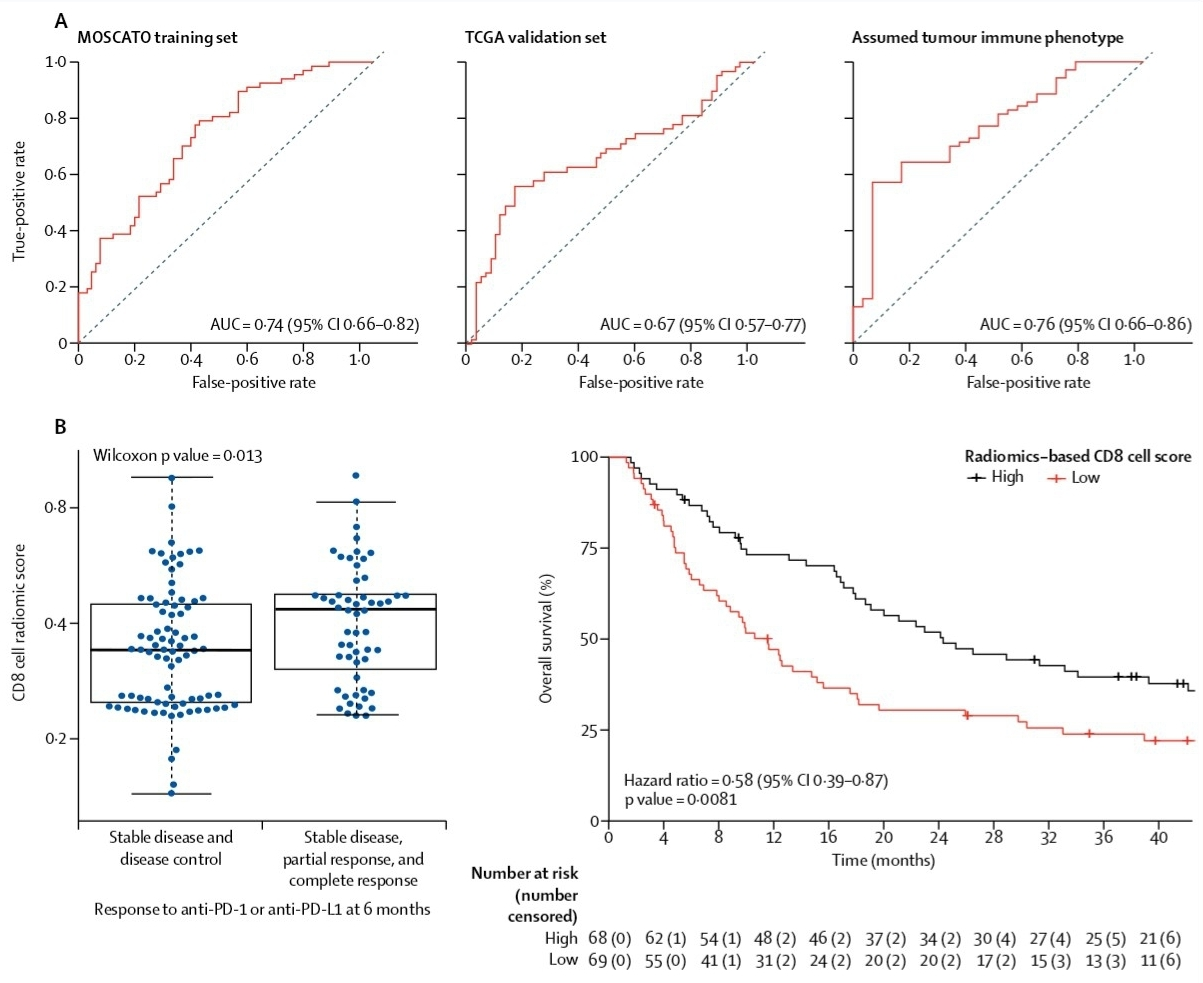
\includegraphics[width=0.5\textwidth]{figures/figure3 cropped.jpg}
      \caption{Performance of the radiomic signature in training and validation datasets, from \cite{main}.}
\end{figure}

\subsection{Radiomic Signature Performance (Genomic and Phenotypic Validation)}
In the MOSCATO training dataset, the elastic-net derived radiomic score successfully discriminated between high and low CD8 cell infiltration (based on the gene expression median) with an Area Under the Curve (AUC) of $0.74$ ($95\%$ CI: $0.66$-$0.82$).

When applied to the completely independent, multi-centre TCGA validation set, the signature achieved an AUC of $0.67$ ($95\%$ CI: $0.57$-$0.77$). From a critical perspective, while statistically significant, an AUC of $0.67$ demonstrates only moderate discriminative ability. This highlights the inherent difficulty of applying an imaging biomarker trained on one specific dataset to a highly heterogeneous, external dataset spanning multiple cancer types and imaging protocols. However, the authors' sensitivity analysis confirmed that without the non-radiomic variables (like peak kilovoltage and tumour location), the performance in the TCGA cohort dropped further, underscoring the necessity of these parameters.

In the immune phenotype cohort, the radiomic score effectively discriminated between clinically assumed "immune-inflamed" and "immune-desert" tumours, achieving an AUC of $0.76$ ($95\%$ CI: $0.66$-$0.86$). While promising, this result should be interpreted with caution, as the phenotypic labels were assumed based on tumour histology rather than confirmed by pathological assessment.

\subsection{Concordance with Pathology}
To verify that the radiomic score correlated with actual immune cells rather than just a surrogate gene signature, the authors compared the score to a pathologist's quantification of tumour-infiltrating lymphocytes in a subset of $77$ TCGA patients. When pooling four cancer types (bladder, lung adenocarcinoma, lung squamous, and liver), they found a significant correlation (Spearman's $\rho = 0.559$, $p = 0.00022$).

Crucially, however, the correlation completely failed in the head and neck squamous cell carcinoma (HNSC) subgroup ($p = 0.18$). The authors had to perform a post-hoc analysis regrouping various head and neck tumours to achieve significant discrimination. This inconsistency suggests the biomarker may not generalize well to all tissue types.

\subsection{Clinical Outcomes in the Immunotherapy Cohort}
The biomarker was applied to the cohort of $137$ patients treated with anti-PD-1 or anti-PD-L1 therapies.
\paragraph{Objective Response.} Continuous baseline radiomic scores (not binarized, unlike the survival analysis) were shown to be significantly higher (via Wilcoxon rank-sum test) in patients achieving an objective response at $3$ months ($p=0.049$) and $6$ months ($p=0.025$).
\paragraph{Overall Survival (OS).} Patients categorized in the "high" radiomic score group exhibited vastly improved survival. The median OS was $24.3$ months for the high-score group compared to $11.5$ months for the low-score group. The radiomic score proved to be a strong prognostic factor in univariate (HR $0.58$) and multivariate analyses (HR $0.52$).

\subsection{Critical Limitations of the Clinical Results}
While the survival curves are compelling, two major confounding factors must be addressed. First, all patients with liver lesions clustered exclusively into the low radiomic score group. While biologically consistent with known poor CD8 infiltration in liver metastases, this acts as a major uncontrolled clinical confounder for survival analysis. Second, the authors clustered patients into "high" and "low" survival groups by binarizing the data exactly at the median radiomic score. Deciding a cutoff threshold post-hoc based on the median of the current dataset risks introducing optimistic bias, meaning the survival differences might appear more dramatic here than they would in a truly prospective, pre-defined trial.


% ==============================================================================
% SECTION : CONCLUSION AND DISCUSSION
% ==============================================================================
\section{Conclusion and Discussion}
The study by Sun et al. \cite{main} represents a significant and innovative step forward in precision oncology. By successfully developing a non-invasive radiomic signature to predict CD8+ T-cell infiltration, the authors provided a promising framework to infer clinical outcomes for patients treated with anti-PD-1 and anti-PD-L1 immunotherapy.

\subsection{Methodological Strengths}
The study's architecture is highly commendable. Its primary strength lies in the robust, four-cohort design, which leverages three truly independent validation sets. This statistically sound approach heavily mitigates the risk of overfitting to a specific tumour subset. Furthermore, the authors made biologically motivated choices, such as generating a $4$ mm peripheral ring to capture the tumour microenvironment, and utilized an elastic-net regression model for principled, heavily penalized feature selection. Their sensitivity analyses also correctly highlighted the necessity of including technical variables, like peak kilovoltage (kVp) and tumour location, to correct for inter-scanner and tissue variability across heterogeneous datasets.

\subsection{Critical Limitations}
Despite these strengths, our critique reveals several methodological constraints that must be considered:
\paragraph{Surrogate Outcomes and Inference Chains.} The model does not predict CD8 cell counts but rather the MCPcounter-derived estimate of CD8 cell abundance (based on the CD8B gene), which is itself a surrogate for CD8 infiltration. This creates a chain of untested assumptions, as the gene signature may not perfectly reflect true cellular abundance, and the radiomic features may not perfectly capture the gene expression.
\paragraph{Data Quantification Mismatch.} There is a fundamental discrepancy in how the RNA-sequencing data was quantified. The MOSCATO training set used Transcripts Per Million (TPM), while the TCGA validation set used Reads Per Kilobase Million (RPKM). Though the authors attempted to correct this by rescaling the data to match the training set's mean and variance stratified by location, harmonizing different transcriptomic quantification methods inherently introduces noise.
\paragraph{Clinical Confounders and Optimistic Bias.} The immunotherapy survival outcomes were evaluated retrospectively using a post-hoc median threshold to binarize patients into "high" and "low" groups, which means the threshold cannot be applied prospectively to a new cohort without recalibration. Additionally, all patients with liver lesions, a site known for poor immunotherapy response \cite{tumeh2017}, clustered entirely into the low radiomic score group, acting as a major uncontrolled clinical confounder.
\paragraph{Lack of Calibration.} The study reports only on the model's discriminative ability (via AUC metrics) and entirely omits calibration metrics, which are crucial for understanding how well the predicted probabilities match actual observed event rates. It also fails to report positive or negative predictive values that would tell a clinician the actual probability of a patient responding in such an imbalanced clinical setting.

\subsection{Future Extensions}
To transition this biomarker from an exploratory research tool to a clinically actionable test, the next step should be prospective validation in large, standardized randomized controlled trials. Future iterations of this model should aim to establish strict, pre-defined predictive thresholds rather than relying on retrospective medians. Additionally, as our understanding of the tumour microenvironment evolves, models should be extended to incorporate more complex immunological subtypes beyond the binary "inflamed" vs "desert" paradigm, and standardizing image acquisition protocols will remain essential for reproducibility. Furthermore, tissue-specific recalibration should be explored, given the biomarker's failure to correlate with pathology in the HNSC subgroup.


% ==============================================================================
% SECTION : BIBLIOGRAPHY
% ==============================================================================
\printbibliography


% ==============================================================================
% SECTION : APPENDIX
% ==============================================================================
% \newpage
% \appendix
% \section{Appendix: Appendix section}\label{sec:appendix}


\end{document}